Across all non-mean regressors and split strategies, frozen ESM-2 embeddings achieved lower test MAE than handcrafted sequence features. On the generated random split, the best ESM-2 model was random forest regression with MAE 0.6250 and 95\% bootstrap CI [0.5930, 0.6574]. The corresponding handcrafted random forest model had MAE 0.6984. On the MMseqs2 90\% cluster-safe split, the best ESM-2 model was histogram gradient boosting with MAE 0.6148 and 95\% bootstrap CI [0.5826, 0.6474]. The corresponding handcrafted histogram gradient boosting model had MAE 0.7052.

The current 90\% cluster-safe split did not produce the expected degradation relative to the generated random split. For example, ESM-2 random forest regression had MAE 0.6250 on the generated random split and 0.6164 on the 90\% cluster-safe split. ESM-2 histogram gradient boosting had MAE 0.6335 on the generated random split and 0.6148 on the 90\% cluster-safe split. These results do not support a strong leakage penalty at the 90\% sequence-identity clustering threshold, but they should not be interpreted as evidence that leakage is unimportant. At lower identities, ESM-2 histogram gradient boosting reached MAE 0.6282 at 70\% and 0.6822 at 50\%, showing the expected degradation as the held-out sequences become more distant.

The organism-held-out split also showed lower MAE than the generated random split. ESM-2 random forest regression achieved MAE 0.5360 with 95\% bootstrap CI [0.5079, 0.5609], and ESM-2 histogram gradient boosting achieved MAE 0.5386 with 95\% bootstrap CI [0.5111, 0.5636]. However, the organism-held-out test set had a narrower target distribution than the generated random test set: the target-pH standard deviation was 0.9477 for the organism-held-out test set versus 1.1845 for the generated random test set. This difference likely contributes to the lower MAE and should be considered when interpreting organism generalization.

On the EC-held-out split, ESM-2 random forest achieved the best test MAE at 0.8321 with 95\% bootstrap CI [0.7913, 0.8773]. ESM-2 ridge regression achieved MAE 0.8395 [0.8028, 0.8808], while the best handcrafted model, random forest, achieved MAE 0.8844. The higher EC-held-out errors indicate that generalization across enzyme classes is harder than the current random and sequence-cluster evaluations.

Paired test-set comparisons of absolute error showed lower error for ESM-2 embeddings than handcrafted features for all non-mean regressors across all available split strategies. Wilcoxon test results were written to \texttt{outputs/metrics/paired\_feature\_group\_comparisons.csv}. Holm--Bonferroni adjustment was applied across the full family of 32 paired tests; all 24 non-mean comparisons remained significant at adjusted \(\alpha=0.05\), while mean-predictor comparisons were unchanged because their paired errors are identical.

\begin{figure}[htbp]
    \centering
    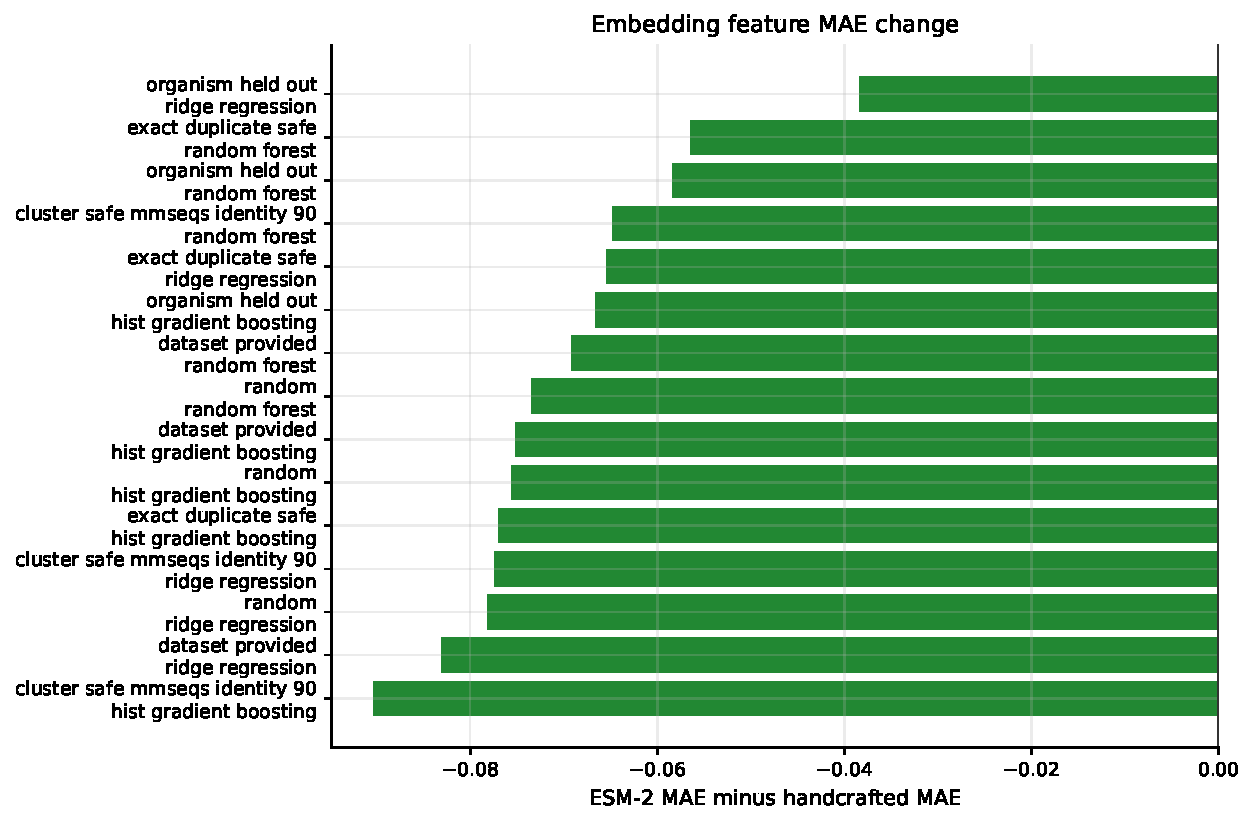
\includegraphics[width=\textwidth]{figures/embedding_vs_handcrafted_mae_change.pdf}
    \caption{Change in test MAE when replacing handcrafted sequence features with frozen ESM-2 embeddings. Negative values indicate lower MAE for embeddings.}
    \label{fig:embedding-vs-handcrafted}
\end{figure}

\begin{figure}[htbp]
    \centering
    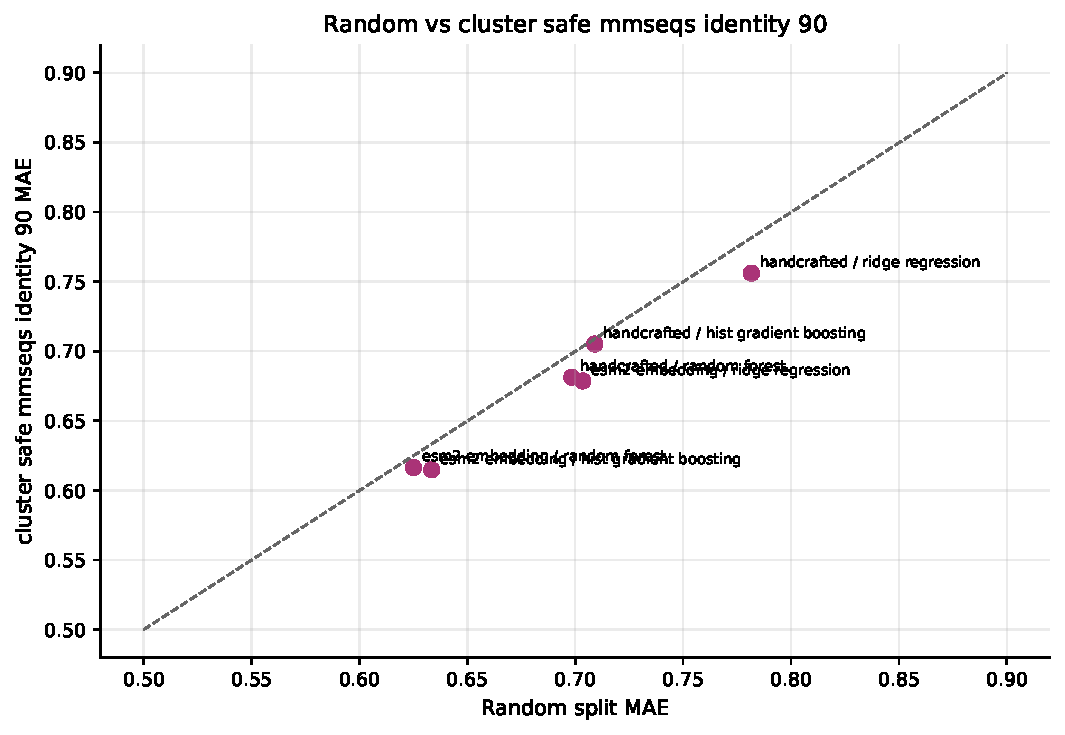
\includegraphics[width=0.78\textwidth]{figures/random_vs_cluster_mae.pdf}
    \caption{Selected comparison of generated random-split MAE and MMseqs2 90\% cluster-safe split MAE for evaluated models. The 70\% and 50\% cluster-safe results are reported in the text and model-comparison tables but are not plotted here. The dashed line indicates equal MAE under both split strategies.}
    \label{fig:random-vs-cluster}
\end{figure}

\begin{figure}[htbp]
    \centering
    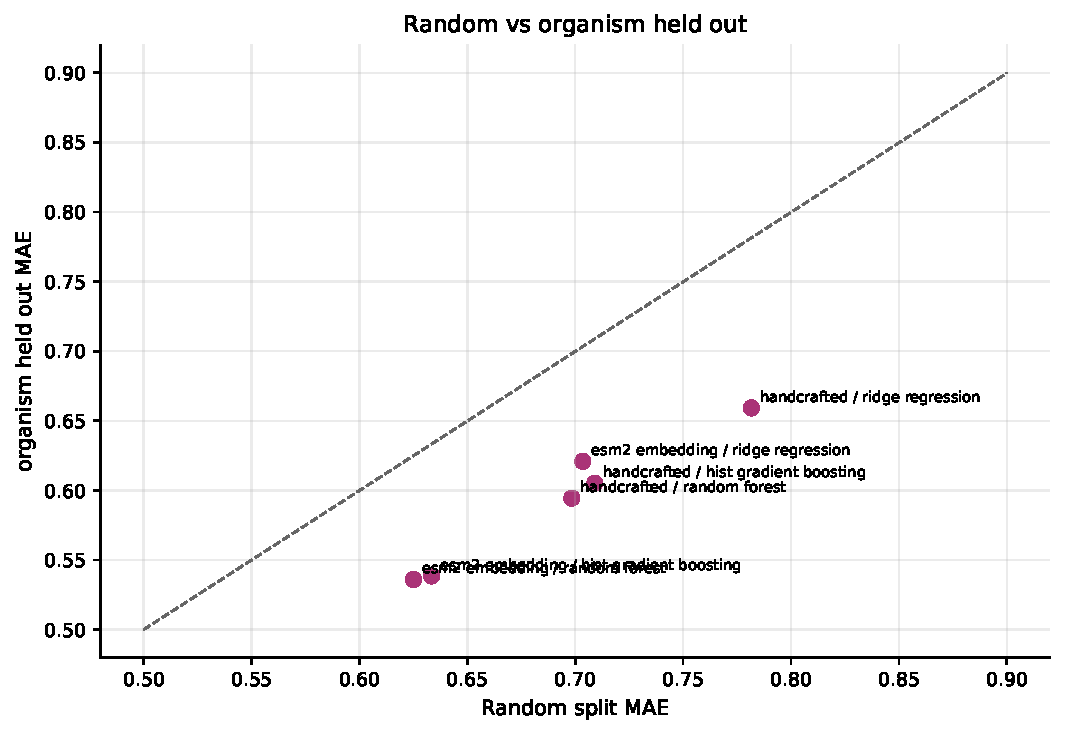
\includegraphics[width=0.78\textwidth]{figures/random_vs_organism_mae.pdf}
    \caption{Selected comparison of generated random-split MAE and organism-held-out split MAE for evaluated models. The cluster-identity and EC-held-out comparisons are reported separately in the text and tables. The organism-held-out test set has a narrower target-pH distribution than the generated random test set.}
    \label{fig:random-vs-organism}
\end{figure}

\begin{figure}[htbp]
    \centering
    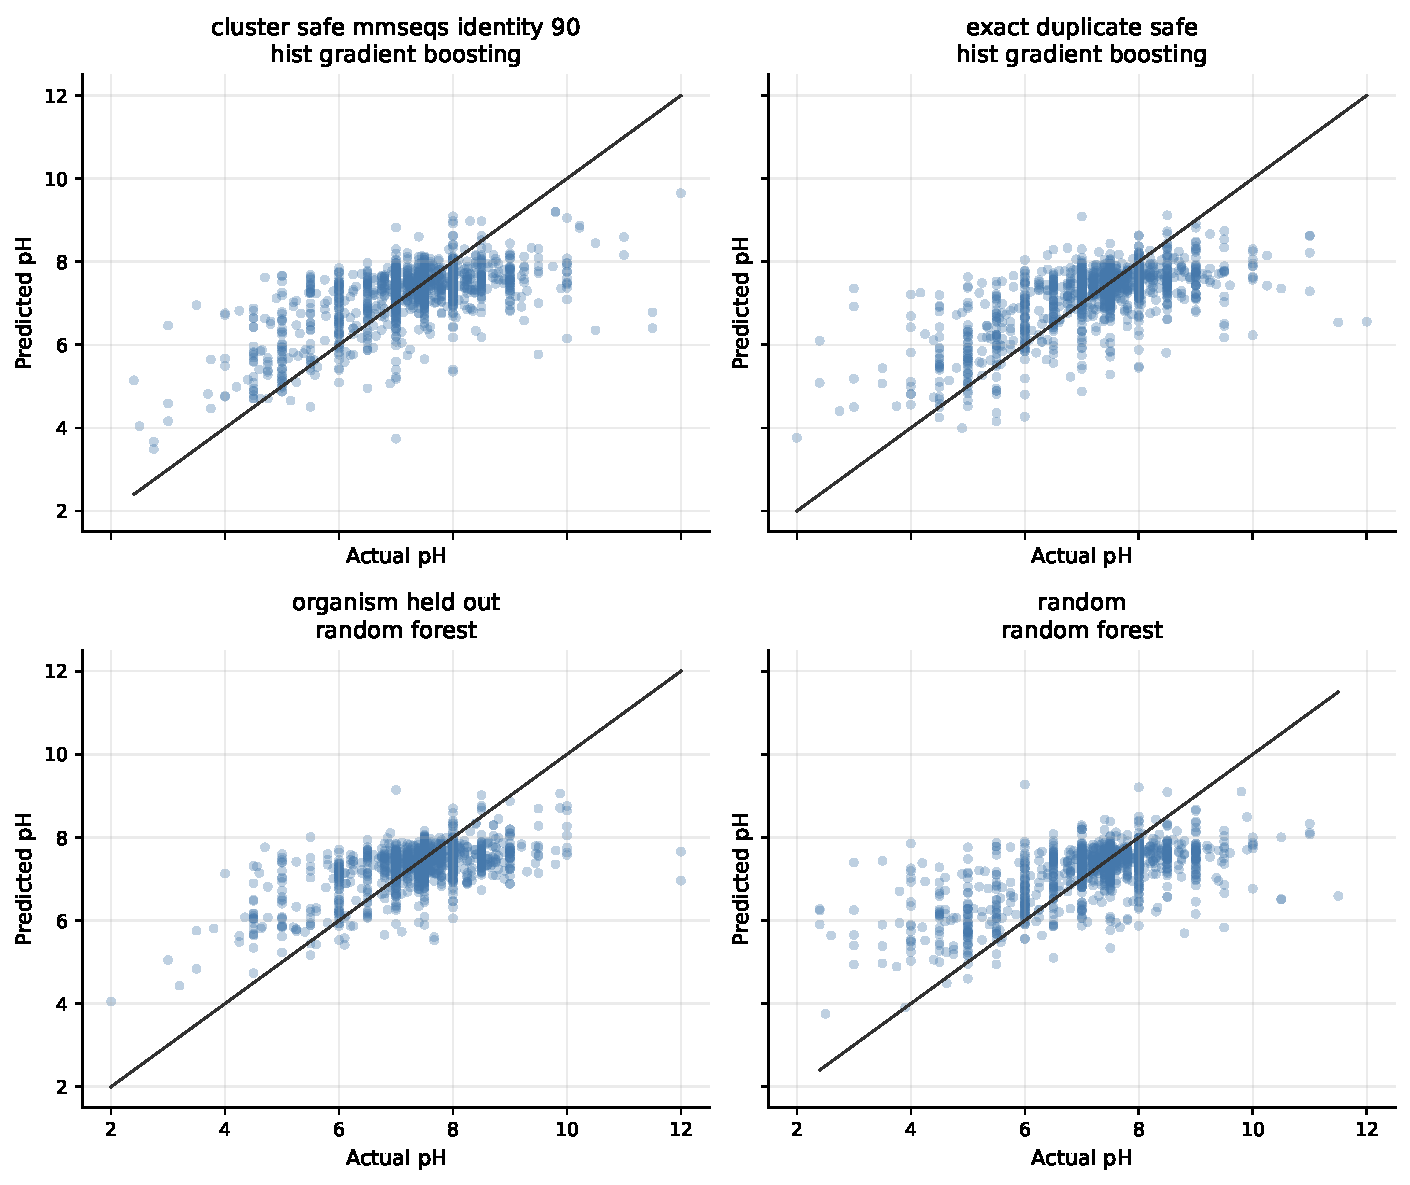
\includegraphics[width=\textwidth]{figures/actual_vs_predicted_best_embedding_models.pdf}
    \caption{Actual versus predicted optimal pH for the selected best ESM-2 embedding models represented in the generated prediction diagnostics. The full set of split-specific metrics, including 50\%, 70\%, and EC-held-out evaluations, is reported in the tables.}
    \label{fig:actual-vs-predicted}
\end{figure}

\begin{longtable}{llllrrrr}
\caption{Test-set performance stratified by experimental optimal-pH range.} \label{tab:performance-by-ph-range} \\
\toprule
feature\_group & split\_strategy & model & ph\_range & n\_examples & mae & rmse & bias \\
\midrule
\endfirsthead
\caption[]{Test-set performance stratified by experimental optimal-pH range.} \\
\toprule
feature\_group & split\_strategy & model & ph\_range & n\_examples & mae & rmse & bias \\
\midrule
\endhead
\midrule
\multicolumn{8}{r}{Continued on next page} \\
\midrule
\endfoot
\bottomrule
\endlastfoot
esm2\_embedding & cluster\_safe\_mmseqs\_identity\_50 & hist\_gradient\_boosting & acidic & 203 & 1.592800 & 1.850100 & 1.578400 \\
esm2\_embedding & cluster\_safe\_mmseqs\_identity\_50 & hist\_gradient\_boosting & alkaline & 174 & 1.303800 & 1.602200 & -1.300900 \\
esm2\_embedding & cluster\_safe\_mmseqs\_identity\_50 & hist\_gradient\_boosting & near\_neutral & 1167 & 0.431100 & 0.582900 & 0.019400 \\
esm2\_embedding & cluster\_safe\_mmseqs\_identity\_50 & mean\_predictor & acidic & 203 & 2.436900 & 2.580400 & 2.436900 \\
esm2\_embedding & cluster\_safe\_mmseqs\_identity\_50 & mean\_predictor & alkaline & 174 & 1.569500 & 1.716700 & -1.569500 \\
esm2\_embedding & cluster\_safe\_mmseqs\_identity\_50 & mean\_predictor & near\_neutral & 1167 & 0.468000 & 0.578800 & -0.027400 \\
esm2\_embedding & cluster\_safe\_mmseqs\_identity\_50 & median\_predictor & acidic & 203 & 2.669300 & 2.800900 & 2.669300 \\
esm2\_embedding & cluster\_safe\_mmseqs\_identity\_50 & median\_predictor & alkaline & 174 & 1.337100 & 1.507100 & -1.337100 \\
esm2\_embedding & cluster\_safe\_mmseqs\_identity\_50 & median\_predictor & near\_neutral & 1167 & 0.426300 & 0.613400 & 0.205000 \\
esm2\_embedding & cluster\_safe\_mmseqs\_identity\_50 & random\_forest & acidic & 203 & 1.655300 & 1.891000 & 1.649100 \\
esm2\_embedding & cluster\_safe\_mmseqs\_identity\_50 & random\_forest & alkaline & 174 & 1.340800 & 1.630600 & -1.340800 \\
esm2\_embedding & cluster\_safe\_mmseqs\_identity\_50 & random\_forest & near\_neutral & 1167 & 0.419300 & 0.568200 & 0.003800 \\
esm2\_embedding & cluster\_safe\_mmseqs\_identity\_50 & ridge\_regression & acidic & 203 & 1.561300 & 1.821200 & 1.545100 \\
esm2\_embedding & cluster\_safe\_mmseqs\_identity\_50 & ridge\_regression & alkaline & 174 & 1.318700 & 1.610900 & -1.316300 \\
esm2\_embedding & cluster\_safe\_mmseqs\_identity\_50 & ridge\_regression & near\_neutral & 1167 & 0.491100 & 0.647300 & -0.002300 \\
esm2\_embedding & cluster\_safe\_mmseqs\_identity\_70 & hist\_gradient\_boosting & acidic & 149 & 1.146300 & 1.453900 & 1.069800 \\
esm2\_embedding & cluster\_safe\_mmseqs\_identity\_70 & hist\_gradient\_boosting & alkaline & 214 & 1.306100 & 1.495500 & -1.301000 \\
esm2\_embedding & cluster\_safe\_mmseqs\_identity\_70 & hist\_gradient\_boosting & near\_neutral & 1118 & 0.429400 & 0.569900 & 0.062600 \\
esm2\_embedding & cluster\_safe\_mmseqs\_identity\_70 & mean\_predictor & acidic & 149 & 2.427800 & 2.559900 & 2.427800 \\
esm2\_embedding & cluster\_safe\_mmseqs\_identity\_70 & mean\_predictor & alkaline & 214 & 1.626200 & 1.736500 & -1.626200 \\
esm2\_embedding & cluster\_safe\_mmseqs\_identity\_70 & mean\_predictor & near\_neutral & 1118 & 0.441800 & 0.543200 & -0.049600 \\
esm2\_embedding & cluster\_safe\_mmseqs\_identity\_70 & median\_predictor & acidic & 149 & 2.696900 & 2.816500 & 2.696900 \\
esm2\_embedding & cluster\_safe\_mmseqs\_identity\_70 & median\_predictor & alkaline & 214 & 1.357000 & 1.487400 & -1.357000 \\
esm2\_embedding & cluster\_safe\_mmseqs\_identity\_70 & median\_predictor & near\_neutral & 1118 & 0.416500 & 0.583800 & 0.219500 \\
esm2\_embedding & cluster\_safe\_mmseqs\_identity\_70 & random\_forest & acidic & 149 & 1.223200 & 1.528000 & 1.199100 \\
esm2\_embedding & cluster\_safe\_mmseqs\_identity\_70 & random\_forest & alkaline & 214 & 1.354100 & 1.530600 & -1.352700 \\
esm2\_embedding & cluster\_safe\_mmseqs\_identity\_70 & random\_forest & near\_neutral & 1118 & 0.412100 & 0.546400 & 0.050200 \\
esm2\_embedding & cluster\_safe\_mmseqs\_identity\_70 & ridge\_regression & acidic & 149 & 1.208000 & 1.478700 & 1.157100 \\
esm2\_embedding & cluster\_safe\_mmseqs\_identity\_70 & ridge\_regression & alkaline & 214 & 1.345300 & 1.538600 & -1.329800 \\
esm2\_embedding & cluster\_safe\_mmseqs\_identity\_70 & ridge\_regression & near\_neutral & 1118 & 0.485800 & 0.619800 & 0.059700 \\
esm2\_embedding & cluster\_safe\_mmseqs\_identity\_90 & hist\_gradient\_boosting & acidic & 152 & 1.170000 & 1.407100 & 1.135700 \\
esm2\_embedding & cluster\_safe\_mmseqs\_identity\_90 & hist\_gradient\_boosting & alkaline & 220 & 1.222100 & 1.441100 & -1.209400 \\
esm2\_embedding & cluster\_safe\_mmseqs\_identity\_90 & hist\_gradient\_boosting & near\_neutral & 1101 & 0.416900 & 0.566000 & 0.044400 \\
esm2\_embedding & cluster\_safe\_mmseqs\_identity\_90 & mean\_predictor & acidic & 152 & 2.326100 & 2.422300 & 2.326100 \\
esm2\_embedding & cluster\_safe\_mmseqs\_identity\_90 & mean\_predictor & alkaline & 220 & 1.624700 & 1.756700 & -1.624700 \\
esm2\_embedding & cluster\_safe\_mmseqs\_identity\_90 & mean\_predictor & near\_neutral & 1101 & 0.448400 & 0.548600 & -0.079200 \\
esm2\_embedding & cluster\_safe\_mmseqs\_identity\_90 & median\_predictor & acidic & 152 & 2.607000 & 2.693200 & 2.607000 \\
esm2\_embedding & cluster\_safe\_mmseqs\_identity\_90 & median\_predictor & alkaline & 220 & 1.343700 & 1.500700 & -1.343700 \\
esm2\_embedding & cluster\_safe\_mmseqs\_identity\_90 & median\_predictor & near\_neutral & 1101 & 0.417600 & 0.579100 & 0.201700 \\
esm2\_embedding & cluster\_safe\_mmseqs\_identity\_90 & random\_forest & acidic & 152 & 1.257900 & 1.483000 & 1.248500 \\
esm2\_embedding & cluster\_safe\_mmseqs\_identity\_90 & random\_forest & alkaline & 220 & 1.276900 & 1.487900 & -1.271700 \\
esm2\_embedding & cluster\_safe\_mmseqs\_identity\_90 & random\_forest & near\_neutral & 1101 & 0.395900 & 0.542700 & 0.033900 \\
esm2\_embedding & cluster\_safe\_mmseqs\_identity\_90 & ridge\_regression & acidic & 152 & 1.239100 & 1.463100 & 1.199300 \\
esm2\_embedding & cluster\_safe\_mmseqs\_identity\_90 & ridge\_regression & alkaline & 220 & 1.307300 & 1.531200 & -1.295500 \\
esm2\_embedding & cluster\_safe\_mmseqs\_identity\_90 & ridge\_regression & near\_neutral & 1101 & 0.475600 & 0.616600 & 0.046100 \\
esm2\_embedding & dataset\_provided & hist\_gradient\_boosting & acidic & 218 & 1.134400 & 1.400400 & 1.055500 \\
esm2\_embedding & dataset\_provided & hist\_gradient\_boosting & alkaline & 285 & 1.178900 & 1.373900 & -1.174000 \\
esm2\_embedding & dataset\_provided & hist\_gradient\_boosting & near\_neutral & 1468 & 0.425900 & 0.573400 & 0.023600 \\
esm2\_embedding & dataset\_provided & mean\_predictor & acidic & 218 & 2.288700 & 2.405900 & 2.288700 \\
esm2\_embedding & dataset\_provided & mean\_predictor & alkaline & 285 & 1.636900 & 1.744600 & -1.636900 \\
esm2\_embedding & dataset\_provided & mean\_predictor & near\_neutral & 1468 & 0.481100 & 0.584000 & -0.072400 \\
esm2\_embedding & dataset\_provided & median\_predictor & acidic & 218 & 2.578000 & 2.682700 & 2.578000 \\
esm2\_embedding & dataset\_provided & median\_predictor & alkaline & 285 & 1.347500 & 1.476500 & -1.347500 \\
esm2\_embedding & dataset\_provided & median\_predictor & near\_neutral & 1468 & 0.442700 & 0.618800 & 0.216900 \\
esm2\_embedding & dataset\_provided & random\_forest & acidic & 218 & 1.172800 & 1.405800 & 1.144900 \\
esm2\_embedding & dataset\_provided & random\_forest & alkaline & 285 & 1.213600 & 1.396400 & -1.213200 \\
esm2\_embedding & dataset\_provided & random\_forest & near\_neutral & 1468 & 0.400500 & 0.544000 & 0.014400 \\
esm2\_embedding & dataset\_provided & ridge\_regression & acidic & 218 & 1.220600 & 1.473000 & 1.153800 \\
esm2\_embedding & dataset\_provided & ridge\_regression & alkaline & 285 & 1.246200 & 1.427300 & -1.234000 \\
esm2\_embedding & dataset\_provided & ridge\_regression & near\_neutral & 1468 & 0.482000 & 0.632600 & 0.011900 \\
esm2\_embedding & ec\_held\_out & hist\_gradient\_boosting & acidic & 360 & 1.351100 & 1.624400 & 1.312000 \\
esm2\_embedding & ec\_held\_out & hist\_gradient\_boosting & alkaline & 138 & 1.875700 & 2.258500 & -1.875700 \\
esm2\_embedding & ec\_held\_out & hist\_gradient\_boosting & near\_neutral & 980 & 0.507700 & 0.683100 & -0.030100 \\
esm2\_embedding & ec\_held\_out & mean\_predictor & acidic & 360 & 2.449400 & 2.544600 & 2.449400 \\
esm2\_embedding & ec\_held\_out & mean\_predictor & alkaline & 138 & 1.677500 & 1.859800 & -1.677500 \\
esm2\_embedding & ec\_held\_out & mean\_predictor & near\_neutral & 980 & 0.522600 & 0.683400 & 0.249400 \\
esm2\_embedding & ec\_held\_out & median\_predictor & acidic & 360 & 2.595800 & 2.685800 & 2.595800 \\
esm2\_embedding & ec\_held\_out & median\_predictor & alkaline & 138 & 1.531100 & 1.728900 & -1.531100 \\
esm2\_embedding & ec\_held\_out & median\_predictor & near\_neutral & 980 & 0.541600 & 0.749400 & 0.395800 \\
esm2\_embedding & ec\_held\_out & random\_forest & acidic & 360 & 1.371000 & 1.620700 & 1.353100 \\
esm2\_embedding & ec\_held\_out & random\_forest & alkaline & 138 & 1.918300 & 2.297400 & -1.918300 \\
esm2\_embedding & ec\_held\_out & random\_forest & near\_neutral & 980 & 0.481200 & 0.650700 & -0.023900 \\
esm2\_embedding & ec\_held\_out & ridge\_regression & acidic & 360 & 1.317800 & 1.556200 & 1.267400 \\
esm2\_embedding & ec\_held\_out & ridge\_regression & alkaline & 138 & 1.881300 & 2.218200 & -1.881200 \\
esm2\_embedding & ec\_held\_out & ridge\_regression & near\_neutral & 980 & 0.517100 & 0.672300 & -0.054500 \\
esm2\_embedding & exact\_duplicate\_safe & hist\_gradient\_boosting & acidic & 174 & 1.091700 & 1.348400 & 1.005200 \\
esm2\_embedding & exact\_duplicate\_safe & hist\_gradient\_boosting & alkaline & 217 & 1.189500 & 1.431300 & -1.179500 \\
esm2\_embedding & exact\_duplicate\_safe & hist\_gradient\_boosting & near\_neutral & 1089 & 0.407800 & 0.558800 & 0.027800 \\
esm2\_embedding & exact\_duplicate\_safe & mean\_predictor & acidic & 174 & 2.268400 & 2.378400 & 2.268400 \\
esm2\_embedding & exact\_duplicate\_safe & mean\_predictor & alkaline & 217 & 1.606000 & 1.732900 & -1.606000 \\
esm2\_embedding & exact\_duplicate\_safe & mean\_predictor & near\_neutral & 1089 & 0.455300 & 0.552400 & -0.084300 \\
esm2\_embedding & exact\_duplicate\_safe & median\_predictor & acidic & 174 & 2.546800 & 2.645200 & 2.546800 \\
esm2\_embedding & exact\_duplicate\_safe & median\_predictor & alkaline & 217 & 1.327600 & 1.478600 & -1.327600 \\
esm2\_embedding & exact\_duplicate\_safe & median\_predictor & near\_neutral & 1089 & 0.413600 & 0.579400 & 0.194100 \\
esm2\_embedding & exact\_duplicate\_safe & random\_forest & acidic & 174 & 1.173300 & 1.410800 & 1.143400 \\
esm2\_embedding & exact\_duplicate\_safe & random\_forest & alkaline & 217 & 1.231900 & 1.476300 & -1.225600 \\
esm2\_embedding & exact\_duplicate\_safe & random\_forest & near\_neutral & 1089 & 0.392400 & 0.529500 & 0.010100 \\
esm2\_embedding & exact\_duplicate\_safe & ridge\_regression & acidic & 174 & 1.250600 & 1.489300 & 1.160800 \\
esm2\_embedding & exact\_duplicate\_safe & ridge\_regression & alkaline & 217 & 1.283600 & 1.538300 & -1.269000 \\
esm2\_embedding & exact\_duplicate\_safe & ridge\_regression & near\_neutral & 1089 & 0.477100 & 0.619800 & -0.003600 \\
esm2\_embedding & organism\_held\_out & hist\_gradient\_boosting & acidic & 88 & 1.334900 & 1.538400 & 1.312700 \\
esm2\_embedding & organism\_held\_out & hist\_gradient\_boosting & alkaline & 209 & 1.069200 & 1.230100 & -1.046900 \\
esm2\_embedding & organism\_held\_out & hist\_gradient\_boosting & near\_neutral & 1181 & 0.385300 & 0.517200 & 0.049000 \\
esm2\_embedding & organism\_held\_out & mean\_predictor & acidic & 88 & 2.274800 & 2.369300 & 2.274800 \\
esm2\_embedding & organism\_held\_out & mean\_predictor & alkaline & 209 & 1.564500 & 1.656800 & -1.564500 \\
esm2\_embedding & organism\_held\_out & mean\_predictor & near\_neutral & 1181 & 0.442100 & 0.532000 & -0.175400 \\
esm2\_embedding & organism\_held\_out & median\_predictor & acidic & 88 & 2.509000 & 2.595000 & 2.509000 \\
esm2\_embedding & organism\_held\_out & median\_predictor & alkaline & 209 & 1.330300 & 1.437800 & -1.330300 \\
esm2\_embedding & organism\_held\_out & median\_predictor & near\_neutral & 1181 & 0.366800 & 0.505600 & 0.058700 \\
esm2\_embedding & organism\_held\_out & random\_forest & acidic & 88 & 1.418900 & 1.596600 & 1.405900 \\
esm2\_embedding & organism\_held\_out & random\_forest & alkaline & 209 & 1.122900 & 1.270000 & -1.111900 \\
esm2\_embedding & organism\_held\_out & random\_forest & near\_neutral & 1181 & 0.366400 & 0.494500 & 0.020100 \\
esm2\_embedding & organism\_held\_out & ridge\_regression & acidic & 88 & 1.408800 & 1.575100 & 1.394900 \\
esm2\_embedding & organism\_held\_out & ridge\_regression & alkaline & 209 & 1.101100 & 1.317600 & -1.069500 \\
esm2\_embedding & organism\_held\_out & ridge\_regression & near\_neutral & 1181 & 0.477200 & 0.617300 & 0.056400 \\
esm2\_embedding & random & hist\_gradient\_boosting & acidic & 177 & 1.280800 & 1.577900 & 1.248800 \\
esm2\_embedding & random & hist\_gradient\_boosting & alkaline & 200 & 1.240100 & 1.448100 & -1.230700 \\
esm2\_embedding & random & hist\_gradient\_boosting & near\_neutral & 1102 & 0.419400 & 0.570800 & 0.044900 \\
esm2\_embedding & random & mean\_predictor & acidic & 177 & 2.442200 & 2.556400 & 2.442200 \\
esm2\_embedding & random & mean\_predictor & alkaline & 200 & 1.592800 & 1.702700 & -1.592800 \\
esm2\_embedding & random & mean\_predictor & near\_neutral & 1102 & 0.452000 & 0.553600 & -0.079100 \\
esm2\_embedding & random & median\_predictor & acidic & 177 & 2.711200 & 2.814500 & 2.711200 \\
esm2\_embedding & random & median\_predictor & alkaline & 200 & 1.323800 & 1.454200 & -1.323800 \\
esm2\_embedding & random & median\_predictor & near\_neutral & 1102 & 0.415000 & 0.579900 & 0.189900 \\
esm2\_embedding & random & random\_forest & acidic & 177 & 1.363300 & 1.638500 & 1.345700 \\
esm2\_embedding & random & random\_forest & alkaline & 200 & 1.266000 & 1.475800 & -1.258700 \\
esm2\_embedding & random & random\_forest & near\_neutral & 1102 & 0.390100 & 0.536900 & 0.016300 \\
esm2\_embedding & random & ridge\_regression & acidic & 177 & 1.459900 & 1.740700 & 1.414200 \\
esm2\_embedding & random & ridge\_regression & alkaline & 200 & 1.297600 & 1.503000 & -1.286100 \\
esm2\_embedding & random & ridge\_regression & near\_neutral & 1102 & 0.474200 & 0.615900 & 0.028500 \\
handcrafted & cluster\_safe\_mmseqs\_identity\_50 & hist\_gradient\_boosting & acidic & 203 & 1.770000 & 2.032000 & 1.743000 \\
handcrafted & cluster\_safe\_mmseqs\_identity\_50 & hist\_gradient\_boosting & alkaline & 174 & 1.398600 & 1.664500 & -1.398600 \\
handcrafted & cluster\_safe\_mmseqs\_identity\_50 & hist\_gradient\_boosting & near\_neutral & 1167 & 0.464100 & 0.612600 & 0.022300 \\
handcrafted & cluster\_safe\_mmseqs\_identity\_50 & mean\_predictor & acidic & 203 & 2.436900 & 2.580400 & 2.436900 \\
handcrafted & cluster\_safe\_mmseqs\_identity\_50 & mean\_predictor & alkaline & 174 & 1.569500 & 1.716700 & -1.569500 \\
handcrafted & cluster\_safe\_mmseqs\_identity\_50 & mean\_predictor & near\_neutral & 1167 & 0.468000 & 0.578800 & -0.027400 \\
handcrafted & cluster\_safe\_mmseqs\_identity\_50 & median\_predictor & acidic & 203 & 2.669300 & 2.800900 & 2.669300 \\
handcrafted & cluster\_safe\_mmseqs\_identity\_50 & median\_predictor & alkaline & 174 & 1.337100 & 1.507100 & -1.337100 \\
handcrafted & cluster\_safe\_mmseqs\_identity\_50 & median\_predictor & near\_neutral & 1167 & 0.426300 & 0.613400 & 0.205000 \\
handcrafted & cluster\_safe\_mmseqs\_identity\_50 & random\_forest & acidic & 203 & 1.811000 & 2.057100 & 1.793900 \\
handcrafted & cluster\_safe\_mmseqs\_identity\_50 & random\_forest & alkaline & 174 & 1.415900 & 1.668000 & -1.415900 \\
handcrafted & cluster\_safe\_mmseqs\_identity\_50 & random\_forest & near\_neutral & 1167 & 0.449700 & 0.588700 & 0.013700 \\
handcrafted & cluster\_safe\_mmseqs\_identity\_50 & ridge\_regression & acidic & 203 & 1.968400 & 2.185500 & 1.968400 \\
handcrafted & cluster\_safe\_mmseqs\_identity\_50 & ridge\_regression & alkaline & 174 & 1.462400 & 1.699400 & -1.455300 \\
handcrafted & cluster\_safe\_mmseqs\_identity\_50 & ridge\_regression & near\_neutral & 1167 & 0.463400 & 0.599700 & -0.001500 \\
handcrafted & cluster\_safe\_mmseqs\_identity\_70 & hist\_gradient\_boosting & acidic & 149 & 1.540300 & 1.794400 & 1.505600 \\
handcrafted & cluster\_safe\_mmseqs\_identity\_70 & hist\_gradient\_boosting & alkaline & 214 & 1.442800 & 1.612100 & -1.442800 \\
handcrafted & cluster\_safe\_mmseqs\_identity\_70 & hist\_gradient\_boosting & near\_neutral & 1118 & 0.447700 & 0.586000 & 0.035800 \\
handcrafted & cluster\_safe\_mmseqs\_identity\_70 & mean\_predictor & acidic & 149 & 2.427800 & 2.559900 & 2.427800 \\
handcrafted & cluster\_safe\_mmseqs\_identity\_70 & mean\_predictor & alkaline & 214 & 1.626200 & 1.736500 & -1.626200 \\
handcrafted & cluster\_safe\_mmseqs\_identity\_70 & mean\_predictor & near\_neutral & 1118 & 0.441800 & 0.543200 & -0.049600 \\
handcrafted & cluster\_safe\_mmseqs\_identity\_70 & median\_predictor & acidic & 149 & 2.696900 & 2.816500 & 2.696900 \\
handcrafted & cluster\_safe\_mmseqs\_identity\_70 & median\_predictor & alkaline & 214 & 1.357000 & 1.487400 & -1.357000 \\
handcrafted & cluster\_safe\_mmseqs\_identity\_70 & median\_predictor & near\_neutral & 1118 & 0.416500 & 0.583800 & 0.219500 \\
handcrafted & cluster\_safe\_mmseqs\_identity\_70 & random\_forest & acidic & 149 & 1.555300 & 1.819600 & 1.530600 \\
handcrafted & cluster\_safe\_mmseqs\_identity\_70 & random\_forest & alkaline & 214 & 1.477100 & 1.653900 & -1.477100 \\
handcrafted & cluster\_safe\_mmseqs\_identity\_70 & random\_forest & near\_neutral & 1118 & 0.431100 & 0.565600 & 0.020400 \\
handcrafted & cluster\_safe\_mmseqs\_identity\_70 & ridge\_regression & acidic & 149 & 1.832900 & 2.031800 & 1.832900 \\
handcrafted & cluster\_safe\_mmseqs\_identity\_70 & ridge\_regression & alkaline & 214 & 1.545700 & 1.713400 & -1.542800 \\
handcrafted & cluster\_safe\_mmseqs\_identity\_70 & ridge\_regression & near\_neutral & 1118 & 0.453300 & 0.573100 & -0.021800 \\
handcrafted & cluster\_safe\_mmseqs\_identity\_90 & hist\_gradient\_boosting & acidic & 152 & 1.445900 & 1.652200 & 1.408100 \\
handcrafted & cluster\_safe\_mmseqs\_identity\_90 & hist\_gradient\_boosting & alkaline & 220 & 1.391300 & 1.603600 & -1.389600 \\
handcrafted & cluster\_safe\_mmseqs\_identity\_90 & hist\_gradient\_boosting & near\_neutral & 1101 & 0.465800 & 0.620800 & 0.043500 \\
handcrafted & cluster\_safe\_mmseqs\_identity\_90 & mean\_predictor & acidic & 152 & 2.326100 & 2.422300 & 2.326100 \\
handcrafted & cluster\_safe\_mmseqs\_identity\_90 & mean\_predictor & alkaline & 220 & 1.624700 & 1.756700 & -1.624700 \\
handcrafted & cluster\_safe\_mmseqs\_identity\_90 & mean\_predictor & near\_neutral & 1101 & 0.448400 & 0.548600 & -0.079200 \\
handcrafted & cluster\_safe\_mmseqs\_identity\_90 & median\_predictor & acidic & 152 & 2.607000 & 2.693200 & 2.607000 \\
handcrafted & cluster\_safe\_mmseqs\_identity\_90 & median\_predictor & alkaline & 220 & 1.343700 & 1.500700 & -1.343700 \\
handcrafted & cluster\_safe\_mmseqs\_identity\_90 & median\_predictor & near\_neutral & 1101 & 0.417600 & 0.579100 & 0.201700 \\
handcrafted & cluster\_safe\_mmseqs\_identity\_90 & random\_forest & acidic & 152 & 1.477800 & 1.674400 & 1.464900 \\
handcrafted & cluster\_safe\_mmseqs\_identity\_90 & random\_forest & alkaline & 220 & 1.387400 & 1.601300 & -1.385000 \\
handcrafted & cluster\_safe\_mmseqs\_identity\_90 & random\_forest & near\_neutral & 1101 & 0.430200 & 0.576900 & 0.020400 \\
handcrafted & cluster\_safe\_mmseqs\_identity\_90 & ridge\_regression & acidic & 152 & 1.769100 & 1.890400 & 1.769100 \\
handcrafted & cluster\_safe\_mmseqs\_identity\_90 & ridge\_regression & alkaline & 220 & 1.480000 & 1.698000 & -1.472100 \\
handcrafted & cluster\_safe\_mmseqs\_identity\_90 & ridge\_regression & near\_neutral & 1101 & 0.471500 & 0.603200 & 0.002000 \\
handcrafted & dataset\_provided & hist\_gradient\_boosting & acidic & 218 & 1.392800 & 1.625900 & 1.345100 \\
handcrafted & dataset\_provided & hist\_gradient\_boosting & alkaline & 285 & 1.346700 & 1.516900 & -1.346100 \\
handcrafted & dataset\_provided & hist\_gradient\_boosting & near\_neutral & 1468 & 0.455800 & 0.598800 & 0.008700 \\
handcrafted & dataset\_provided & mean\_predictor & acidic & 218 & 2.288700 & 2.405900 & 2.288700 \\
handcrafted & dataset\_provided & mean\_predictor & alkaline & 285 & 1.636900 & 1.744600 & -1.636900 \\
handcrafted & dataset\_provided & mean\_predictor & near\_neutral & 1468 & 0.481100 & 0.584000 & -0.072400 \\
handcrafted & dataset\_provided & median\_predictor & acidic & 218 & 2.578000 & 2.682700 & 2.578000 \\
handcrafted & dataset\_provided & median\_predictor & alkaline & 285 & 1.347500 & 1.476500 & -1.347500 \\
handcrafted & dataset\_provided & median\_predictor & near\_neutral & 1468 & 0.442700 & 0.618800 & 0.216900 \\
handcrafted & dataset\_provided & random\_forest & acidic & 218 & 1.380200 & 1.607100 & 1.345300 \\
handcrafted & dataset\_provided & random\_forest & alkaline & 285 & 1.354700 & 1.529900 & -1.354400 \\
handcrafted & dataset\_provided & random\_forest & near\_neutral & 1468 & 0.435200 & 0.578100 & 0.004500 \\
handcrafted & dataset\_provided & ridge\_regression & acidic & 218 & 1.656000 & 1.835000 & 1.656000 \\
handcrafted & dataset\_provided & ridge\_regression & alkaline & 285 & 1.479100 & 1.641700 & -1.476700 \\
handcrafted & dataset\_provided & ridge\_regression & near\_neutral & 1468 & 0.483700 & 0.611800 & -0.017400 \\
handcrafted & ec\_held\_out & hist\_gradient\_boosting & acidic & 360 & 1.570200 & 1.812700 & 1.499100 \\
handcrafted & ec\_held\_out & hist\_gradient\_boosting & alkaline & 138 & 1.757000 & 2.067200 & -1.757000 \\
handcrafted & ec\_held\_out & hist\_gradient\_boosting & near\_neutral & 980 & 0.554100 & 0.717300 & 0.059400 \\
handcrafted & ec\_held\_out & mean\_predictor & acidic & 360 & 2.449400 & 2.544600 & 2.449400 \\
handcrafted & ec\_held\_out & mean\_predictor & alkaline & 138 & 1.677500 & 1.859800 & -1.677500 \\
handcrafted & ec\_held\_out & mean\_predictor & near\_neutral & 980 & 0.522600 & 0.683400 & 0.249400 \\
handcrafted & ec\_held\_out & median\_predictor & acidic & 360 & 2.595800 & 2.685800 & 2.595800 \\
handcrafted & ec\_held\_out & median\_predictor & alkaline & 138 & 1.531100 & 1.728900 & -1.531100 \\
handcrafted & ec\_held\_out & median\_predictor & near\_neutral & 980 & 0.541600 & 0.749400 & 0.395800 \\
handcrafted & ec\_held\_out & random\_forest & acidic & 360 & 1.539600 & 1.780600 & 1.501900 \\
handcrafted & ec\_held\_out & random\_forest & alkaline & 138 & 1.753100 & 2.052800 & -1.753100 \\
handcrafted & ec\_held\_out & random\_forest & near\_neutral & 980 & 0.521400 & 0.675600 & 0.036200 \\
handcrafted & ec\_held\_out & ridge\_regression & acidic & 360 & 1.806700 & 1.946200 & 1.806700 \\
handcrafted & ec\_held\_out & ridge\_regression & alkaline & 138 & 1.807600 & 2.074100 & -1.806900 \\
handcrafted & ec\_held\_out & ridge\_regression & near\_neutral & 980 & 0.490200 & 0.621000 & 0.065900 \\
handcrafted & exact\_duplicate\_safe & hist\_gradient\_boosting & acidic & 174 & 1.361100 & 1.617000 & 1.298200 \\
handcrafted & exact\_duplicate\_safe & hist\_gradient\_boosting & alkaline & 217 & 1.321700 & 1.540800 & -1.321700 \\
handcrafted & exact\_duplicate\_safe & hist\_gradient\_boosting & near\_neutral & 1089 & 0.442900 & 0.587700 & 0.001300 \\
handcrafted & exact\_duplicate\_safe & mean\_predictor & acidic & 174 & 2.268400 & 2.378400 & 2.268400 \\
handcrafted & exact\_duplicate\_safe & mean\_predictor & alkaline & 217 & 1.606000 & 1.732900 & -1.606000 \\
handcrafted & exact\_duplicate\_safe & mean\_predictor & near\_neutral & 1089 & 0.455300 & 0.552400 & -0.084300 \\
handcrafted & exact\_duplicate\_safe & median\_predictor & acidic & 174 & 2.546800 & 2.645200 & 2.546800 \\
handcrafted & exact\_duplicate\_safe & median\_predictor & alkaline & 217 & 1.327600 & 1.478600 & -1.327600 \\
handcrafted & exact\_duplicate\_safe & median\_predictor & near\_neutral & 1089 & 0.413600 & 0.579400 & 0.194100 \\
handcrafted & exact\_duplicate\_safe & random\_forest & acidic & 174 & 1.365600 & 1.629800 & 1.334300 \\
handcrafted & exact\_duplicate\_safe & random\_forest & alkaline & 217 & 1.341500 & 1.561200 & -1.341500 \\
handcrafted & exact\_duplicate\_safe & random\_forest & near\_neutral & 1089 & 0.416600 & 0.549400 & -0.017400 \\
handcrafted & exact\_duplicate\_safe & ridge\_regression & acidic & 174 & 1.654200 & 1.845600 & 1.654200 \\
handcrafted & exact\_duplicate\_safe & ridge\_regression & alkaline & 217 & 1.495600 & 1.696400 & -1.495600 \\
handcrafted & exact\_duplicate\_safe & ridge\_regression & near\_neutral & 1089 & 0.459400 & 0.586100 & -0.040600 \\
handcrafted & organism\_held\_out & hist\_gradient\_boosting & acidic & 88 & 1.693900 & 1.872200 & 1.658700 \\
handcrafted & organism\_held\_out & hist\_gradient\_boosting & alkaline & 209 & 1.214300 & 1.370000 & -1.214300 \\
handcrafted & organism\_held\_out & hist\_gradient\_boosting & near\_neutral & 1181 & 0.416200 & 0.543300 & 0.026600 \\
handcrafted & organism\_held\_out & mean\_predictor & acidic & 88 & 2.274800 & 2.369300 & 2.274800 \\
handcrafted & organism\_held\_out & mean\_predictor & alkaline & 209 & 1.564500 & 1.656800 & -1.564500 \\
handcrafted & organism\_held\_out & mean\_predictor & near\_neutral & 1181 & 0.442100 & 0.532000 & -0.175400 \\
handcrafted & organism\_held\_out & median\_predictor & acidic & 88 & 2.509000 & 2.595000 & 2.509000 \\
handcrafted & organism\_held\_out & median\_predictor & alkaline & 209 & 1.330300 & 1.437800 & -1.330300 \\
handcrafted & organism\_held\_out & median\_predictor & near\_neutral & 1181 & 0.366800 & 0.505600 & 0.058700 \\
handcrafted & organism\_held\_out & random\_forest & acidic & 88 & 1.723700 & 1.900900 & 1.707800 \\
handcrafted & organism\_held\_out & random\_forest & alkaline & 209 & 1.238100 & 1.381300 & -1.238100 \\
handcrafted & organism\_held\_out & random\_forest & near\_neutral & 1181 & 0.396400 & 0.520300 & -0.000100 \\
handcrafted & organism\_held\_out & ridge\_regression & acidic & 88 & 1.851000 & 1.985100 & 1.850400 \\
handcrafted & organism\_held\_out & ridge\_regression & alkaline & 209 & 1.407000 & 1.555300 & -1.407000 \\
handcrafted & organism\_held\_out & ridge\_regression & near\_neutral & 1181 & 0.438100 & 0.556000 & -0.078600 \\
handcrafted & random & hist\_gradient\_boosting & acidic & 177 & 1.501600 & 1.811300 & 1.438300 \\
handcrafted & random & hist\_gradient\_boosting & alkaline & 200 & 1.377800 & 1.583700 & -1.377800 \\
handcrafted & random & hist\_gradient\_boosting & near\_neutral & 1102 & 0.460400 & 0.610800 & 0.012400 \\
handcrafted & random & mean\_predictor & acidic & 177 & 2.442200 & 2.556400 & 2.442200 \\
handcrafted & random & mean\_predictor & alkaline & 200 & 1.592800 & 1.702700 & -1.592800 \\
handcrafted & random & mean\_predictor & near\_neutral & 1102 & 0.452000 & 0.553600 & -0.079100 \\
handcrafted & random & median\_predictor & acidic & 177 & 2.711200 & 2.814500 & 2.711200 \\
handcrafted & random & median\_predictor & alkaline & 200 & 1.323800 & 1.454200 & -1.323800 \\
handcrafted & random & median\_predictor & near\_neutral & 1102 & 0.415000 & 0.579900 & 0.189900 \\
handcrafted & random & random\_forest & acidic & 177 & 1.528200 & 1.831200 & 1.507400 \\
handcrafted & random & random\_forest & alkaline & 200 & 1.405400 & 1.623900 & -1.405400 \\
handcrafted & random & random\_forest & near\_neutral & 1102 & 0.436800 & 0.596400 & 0.000000 \\
handcrafted & random & ridge\_regression & acidic & 177 & 1.876800 & 2.086900 & 1.876800 \\
handcrafted & random & ridge\_regression & alkaline & 200 & 1.490200 & 1.668200 & -1.490200 \\
handcrafted & random & ridge\_regression & near\_neutral & 1102 & 0.477200 & 0.607500 & -0.010000 \\
\end{longtable}

